\documentclass[border=2mm]{standalone}
\usepackage{pgfplots}
\pgfplotsset{compat=newest}
\begin{document}
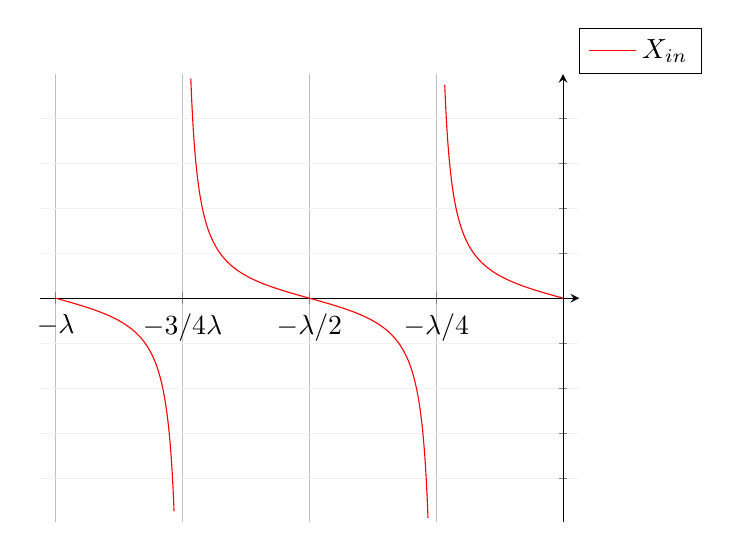
\begin{tikzpicture}
  \begin{axis}%
    [grid=both,
    minor tick num=4,
     grid style={line width=.1pt, draw=gray!10},
     major grid style={line width=.2pt,draw=gray!50},
     axis lines=middle,
     xtick={-2*pi,-3*pi/2,-1*pi,-pi/2, 0},
     ytick={-10,0,10},
     xticklabels={$-\lambda$,$-3/4\lambda$,$-\lambda/2$,$-\lambda/4$,$0$},
    enlargelimits={abs=0.2},
    restrict y to domain=-10:10,    % <-- added
    legend style={at={(1,1)},anchor=south west}
    ]
    \addplot[domain=-2*pi:0,samples=1000,smooth,red] {-tan(deg(x))};
    \addlegendentry{$X_{in}$};
    % \addplot[domain=-2*pi:0,samples=100,smooth,blue] {cos(deg(x))};
    % \addlegendentry{$I(z)$};
  \end{axis}
\end{tikzpicture}   
\end{document}